\chapter{Планиметрия: признаки, центры и дополнительные построения}\label{chap:exam-plane}\markright{Глава 29}

\section{От условия к признаку: прямые и треугольники}
Длины, площади, вписанные углы и степень точки уже введены в главе \ref{chap:plane-geometry}. Здесь важнее распознать достаточное условие: когда равенство углов доказывает параллельность, а свойство диагоналей определяет вид четырёхугольника. Все треугольники далее невырожденные, а четырёхугольники выпуклые; вершины четырёхугольника перечисляются по порядку обхода.

\par\addvspace{2pt}\begin{lrbox}{\CatFlowBox}\begin{minipage}[t]{\linewidth}
\setlength{\parskip}{2pt}\setlength{\columnsep}{4.5mm}\setlength{\intextsep}{0pt}
\begin{wrapfigure}[9]{r}{54mm}
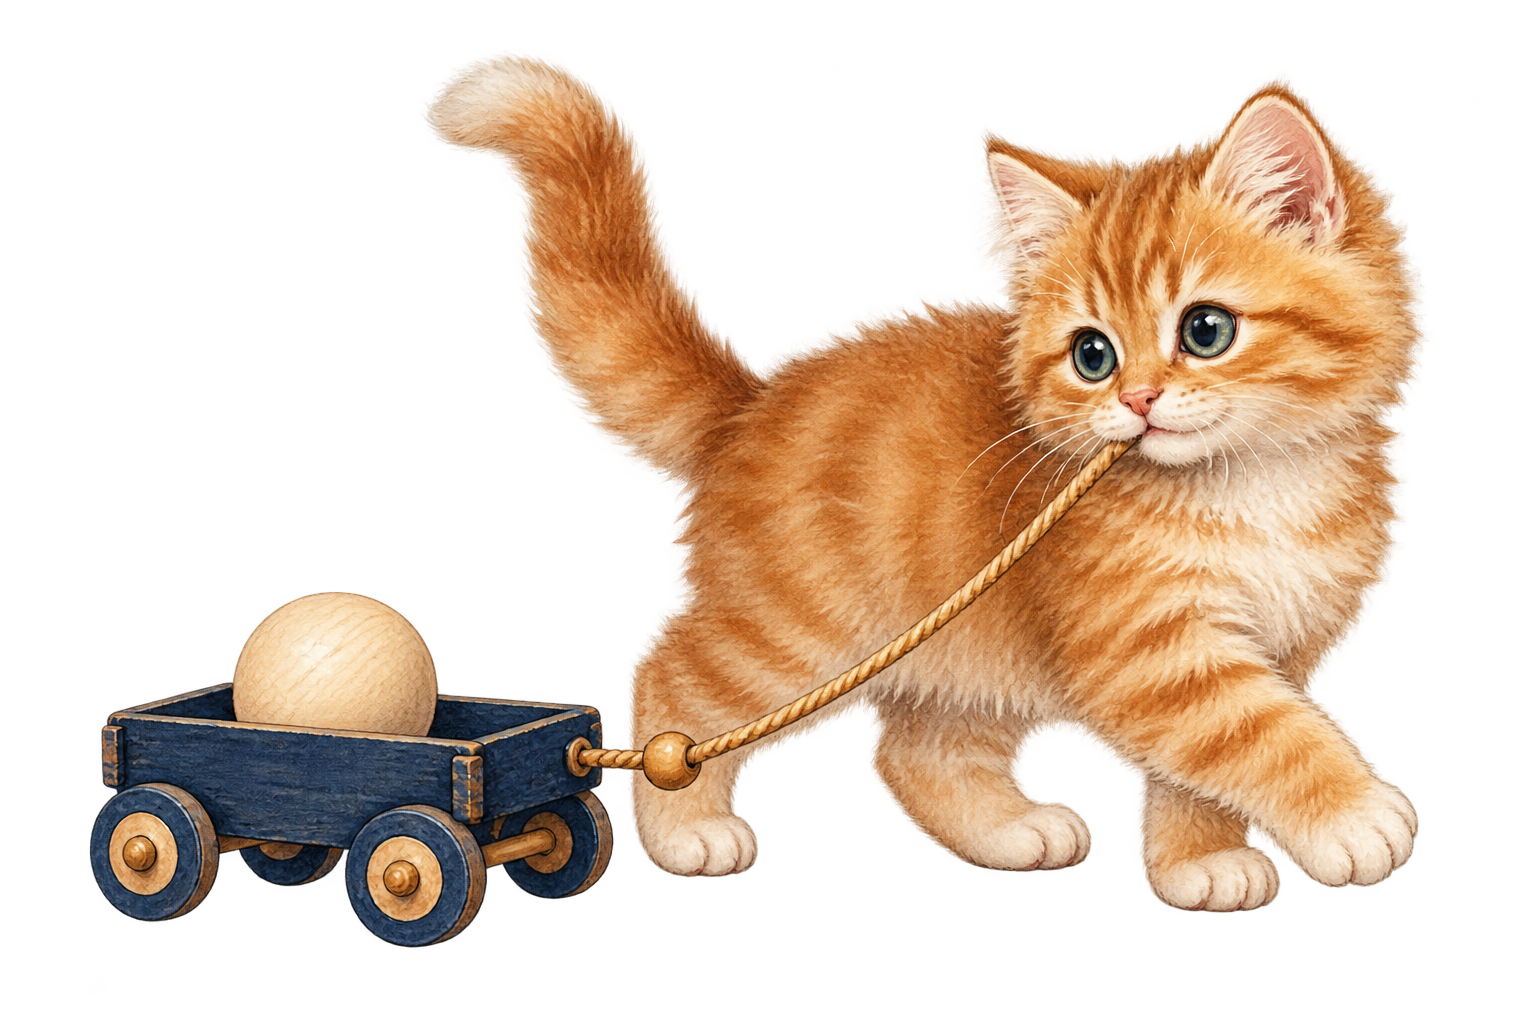
\includegraphics[width=54mm,height=58mm,keepaspectratio]{images/unique/art-242.png}
\end{wrapfigure}
Полезно начинать геометрическое рассуждение с короткого списка данных, которые действительно сообщены в условии. Затем рядом записывают утверждение, которое требуется получить. Между этими двумя списками часто недостаёт всего одного признака: равенства треугольников, параллельности прямых или принадлежности точек одной окружности. На чертеже можно отметить известные равные отрезки одинаковыми штрихами, а известные равные углы одинаковыми дугами. Новые отметки появляются только после обоснования. Если нужного треугольника пока нет, полезно провести диагональ, высоту или параллельную прямую. Такое построение добавляет связь между уже известными величинами. Оно не добавляет произвольного нового условия и не разрешает считать две линии равными лишь потому, что рисунок выглядит симметричным.
\par\WFclear\end{minipage}\end{lrbox}%
\ifdim\dimexpr\ht\CatFlowBox+\dp\CatFlowBox\relax<58mm\dp\CatFlowBox=\dimexpr58mm-\ht\CatFlowBox\relax\fi%
\noindent\usebox{\CatFlowBox}\par\addvspace{2pt}
\begin{definition}\term{Смежные углы} (\emph{adjacent supplementary angles}) имеют общую сторону, а две другие стороны являются противоположными лучами; их сумма равна \(180^\circ\).
\par\term{Вертикальные углы} (\emph{vertical angles}) образованы противоположными лучами двух пересекающихся прямых.
\par При пересечении двух прямых третьей, \term{секущей} (\emph{transversal}), различают \term{соответственные углы} (\emph{corresponding angles}), \term{накрест лежащие углы} (\emph{alternate interior angles}) и \term{односторонние внутренние углы} (\emph{same-side interior angles}). Их положение задаётся сторонами от секущей и расположением внутри или вне полосы между прямыми.\end{definition}
\begin{theorem}[Углы и параллельность]\label{thm:exam-plane-parallel}
Вертикальные углы равны. Для двух различных прямых, пересечённых секущей в различных точках, равносильны: параллельность прямых; равенство пары соответствующих углов; равенство пары накрест лежащих углов; сумма пары односторонних внутренних углов \(180^\circ\).
\end{theorem}
\begin{proof}Два вертикальных угла дополняют один и тот же смежный угол до \(180^\circ\), поэтому равны. Если прямые параллельны, перенос одной точки пересечения в другую вдоль секущей совмещает параллельные прямые и сохраняет углы; соответствующие углы равны. Вертикальные и смежные углы дают остальные два свойства. Обратно, через вторую точку пересечения проведём прямую, параллельную первой. У неё и данной второй прямой совпадает соответствующий угол с тем же лучом секущей. В одной полуплоскости заданный угол определяет единственный луч, значит, прямые совпадают. Случаи накрест лежащих и односторонних углов сводятся к этому вертикальными и смежными углами.\end{proof}

\begin{definition}\term{Равнобедренный треугольник} (\emph{isosceles triangle}) имеет две равные боковые стороны; третья сторона называется основанием.
\par\term{Прямоугольный треугольник} (\emph{right triangle}) имеет прямой угол; противоположная ему сторона — \term{гипотенуза} (\emph{hypotenuse}), остальные две — \term{катеты} (\emph{legs}).\end{definition}
\begin{theorem}[Свойства и признаки равнобедренного треугольника]
Равенство двух сторон равносильно равенству противоположных им углов. В равнобедренном треугольнике биссектриса из вершины между равными сторонами одновременно является медианой и высотой. Если медиана к стороне является высотой, треугольник равнобедренный.
\end{theorem}
\begin{proof}При \(AB=AC\) биссектриса \(AD\) делит треугольник на равные по двум сторонам и углу между ними треугольники \(ABD,ACD\). Отсюда \(BD=DC\), равенство углов при \(B,C\) и равенство смежных углов при \(D\), каждый из которых прямой. Если углы \(B,C\) равны, треугольники \(ABC,ACB\) равны по стороне \(BC\) и прилежащим углам, поэтому \(AB=AC\). Наконец, общая медиана-высота даёт два равных прямоугольных треугольника по двум катетам; гипотенузы \(AB,AC\) равны.\end{proof}
\begin{theorem}[Прямоугольные треугольники]
Два прямоугольных треугольника равны по гипотенузе и катету, по гипотенузе и соответствующему острому углу либо по катету и соответствующему острому углу. Острые углы в сумме дают \(90^\circ\). Катет напротив угла \(30^\circ\) равен половине гипотенузы; верно и обратное.
\end{theorem}
\par\addvspace{2pt}\begin{lrbox}{\CatFlowBox}\begin{minipage}[t]{\linewidth}
\setlength{\parskip}{2pt}\setlength{\columnsep}{4.5mm}\setlength{\intextsep}{0pt}
\begin{wrapfigure}[13]{r}{54mm}

\includegraphics[width=54mm,height=58mm,keepaspectratio]{images/unique/art-257.png}
\end{wrapfigure}
\textit{Доказательство.} В первом признаке Пифагор восстанавливает второй катет, после чего работает равенство по трём сторонам. В остальных признаках прямой и заданный острый углы определяют третий угол; применяем равенство по стороне и двум углам. Сумма острых углов следует из суммы углов треугольника. Отразим прямоугольный треугольник относительно катета, прилежащего к углу \(30^\circ\): получится треугольник с углом \(60^\circ\) между двумя равными гипотенузами, то есть равносторонний. Его третья сторона — удвоенный исходный противолежащий катет. Обратно, если этот катет вдвое меньше гипотенузы, у отражённого треугольника все стороны равны; половина его угла \(60^\circ\) равна \(30^\circ\).\hfill\(\blacksquare\)
\par\WFclear\end{minipage}\end{lrbox}%
\ifdim\dimexpr\ht\CatFlowBox+\dp\CatFlowBox\relax<61mm\dp\CatFlowBox=\dimexpr61mm-\ht\CatFlowBox\relax\fi%
\noindent\usebox{\CatFlowBox}\par\addvspace{2pt}

\begin{theorem}[Неравенство треугольника и существование]
Положительные \(a,b,c\) являются длинами сторон невырожденного треугольника ровно тогда, когда \(|a-b|<c<a+b\). Это равносильно трём строгим неравенствам «сторона меньше суммы двух остальных».
\end{theorem}
\begin{proof}В существующем треугольнике формула косинусов и \(-1<\cos C<1\) дают \((a-b)^2<c^2<(a+b)^2\). Обратно, положим \(A=(0,0),B=(c,0)\). Точка \(C=(x,y)\) с \(AC=b,BC=a\) должна удовлетворять
\[
x=\frac{b^2+c^2-a^2}{2c},\qquad
y^2=\frac{((a+b)^2-c^2)(c^2-(a-b)^2)}{4c^2}.
\]
Условия делают правую часть положительной, поэтому существуют две зеркальные точки \(C\) с \(y\ne0\). При равенстве одной из границ получается только вырожденная фигура на прямой.\end{proof}
\begin{example}\textbf{Разбор 1: угол и признак.} Односторонние углы равны \(3x+15^\circ\) и \(5x+5^\circ\), прямые параллельны. Их сумма \(180^\circ\), поэтому \(8x+20=180\), \(x=20\), углы \(75^\circ,105^\circ\). В треугольнике с двумя равными сторонами угол между ними \(44^\circ\), поэтому каждый угол при основании \(\frac{180-44}{2}=68^\circ\). Обратное рассуждение тоже допустимо: два угла по \(68^\circ\) доказывают равенство противоположных сторон.\end{example}

\section{Подобие, высота и центры треугольника}
\begin{theorem}[Три признака подобия]\label{thm:exam-plane-similarity}
Треугольники подобны: по двум соответствующим углам; по двум пропорциональным соответствующим сторонам и равному углу между ними; по трём пропорциональным соответствующим сторонам. Если коэффициент длин \(k>0\), отношение площадей равно \(k^2\).
\end{theorem}
\begin{proof}Первый признак доказан в главе \ref{chap:plane-geometry}. Для второго построим треугольник с данным углом и сторонами первого треугольника, увеличенными в \(k\) раз. Он совпадает со вторым по признаку равенства «две стороны и угол между ними». Для третьего такое же увеличение совпадает со вторым по трём сторонам. Увеличение сохраняет углы и умножает высоты на \(k\), поэтому площадь, равная половине произведения основания на высоту, умножается на \(k^2\).\end{proof}
\begin{theorem}[Средняя линия и проекции катетов]\label{thm:exam-plane-midline}
Отрезок между серединами двух сторон треугольника параллелен третьей стороне и вдвое меньше неё. В прямоугольном \(ABC\), \(\angle C=90^\circ\), высота \(CH\) к гипотенузе удовлетворяет
\[
AC^2=AB\cdot AH,\qquad BC^2=AB\cdot BH,\qquad CH^2=AH\cdot BH.
\]
\end{theorem}
\begin{proof}Через середину одной стороны проведём параллель к третьей; подобие с коэффициентом \(\frac{1}{2}\) показывает, что она проходит через середину другой стороны и имеет половинную длину. В прямоугольном треугольнике \(ACH,CBH,ABC\) подобны по двум углам. Из пропорций \(\frac{AC}{AB}=\frac{AH}{AC}\), \(\frac{BC}{AB}=\frac{BH}{BC}\), \(\frac{AH}{CH}=\frac{CH}{BH}\) получаем формулы.\end{proof}
\begin{example}\textbf{Разбор 2: высота без лишнего уравнения.} Катеты равны \(9,12\); гипотенуза \(15\). Проекции катетов на неё равны \(\frac{81}{15}=\frac{27}{5}\) и \(\frac{144}{15}=\frac{48}{5}\), их сумма действительно \(15\). Высота равна \(\frac{9\cdot12}{15}=\frac{36}{5}\), поскольку площадь можно записать как \(\frac{9\cdot12}{2}\) и как \(\frac{15h}{2}\). Проверка \(h^2=(\frac{27}{5})(\frac{48}{5})\) согласуется с подобием.\end{example}

\begin{definition}\term{Серединный перпендикуляр} (\emph{perpendicular bisector}) к отрезку проходит через его середину перпендикулярно ему.
\par\term{Центроид} (\emph{centroid}) — точка пересечения медиан.
\par\term{Инцентр} (\emph{incenter}) — центр вписанной окружности.
\par\term{Центр описанной окружности} (\emph{circumcenter}) обозначают \(O\).
\par\term{Ортоцентр} (\emph{orthocenter}) — точка пересечения прямых, содержащих высоты.\end{definition}
\begin{theorem}[Четыре центра]\label{thm:exam-plane-centers}
Медианы пересекаются в одной точке и делятся ею в отношении \(2:1\) от вершины. Внутренние биссектрисы пересекаются в инцентре; серединные перпендикуляры — в центре описанной окружности; прямые высот — в ортоцентре. Последние два центра могут лежать вне треугольника.
\end{theorem}
\begin{proof}Пусть \(M,N\) — середины \(BC,AC\), \(G=AM\cap BN\). Отрезок \(MN\) параллелен \(AB\) и вдвое меньше него. Подобие \(GMN,GAB\) даёт \(\frac{GM}{GA}=\frac{GN}{GB}=\frac{1}{2}\). Повторив рассуждение с третьей медианой, получаем ту же единственную точку на \(AM\).
Точка внутри угла равноудалена от его сторон ровно тогда, когда лежит на внутренней биссектрисе: это следует из равенства прямоугольных треугольников с общей гипотенузой. Поэтому пересечение двух внутренних биссектрис равноудалено и от третьей стороны, лежит на третьей биссектрисе и является центром касающейся всех сторон окружности. Равноудалённость от концов отрезка аналогично характеризует серединный перпендикуляр; пересечение двух таких прямых равноудалено от всех трёх вершин.
Для высот проведём через каждую вершину прямую, параллельную противоположной стороне. Получится внешний треугольник, у которого \(A,B,C\) — середины сторон: это видно из образовавшихся параллелограммов. Прямые высот исходного треугольника являются серединными перпендикулярами внешнего и потому пересекаются в одной точке.\end{proof}
\begin{theorem}[Деление стороны биссектрисой]
Если внутренняя биссектриса \(AD\) встречает \(BC\) в \(D\), то \(\frac{BD}{DC}=\frac{AB}{AC}\). Для инцентра \(I\) выполнено \(\angle BIC=90^\circ+\frac{1}{2}\angle A\).
\end{theorem}
\par\addvspace{2pt}\begin{lrbox}{\CatFlowBox}\begin{minipage}[t]{\linewidth}
\setlength{\parskip}{2pt}\setlength{\columnsep}{4.5mm}\setlength{\intextsep}{0pt}
\begin{wrapfigure}[11]{l}{54mm}
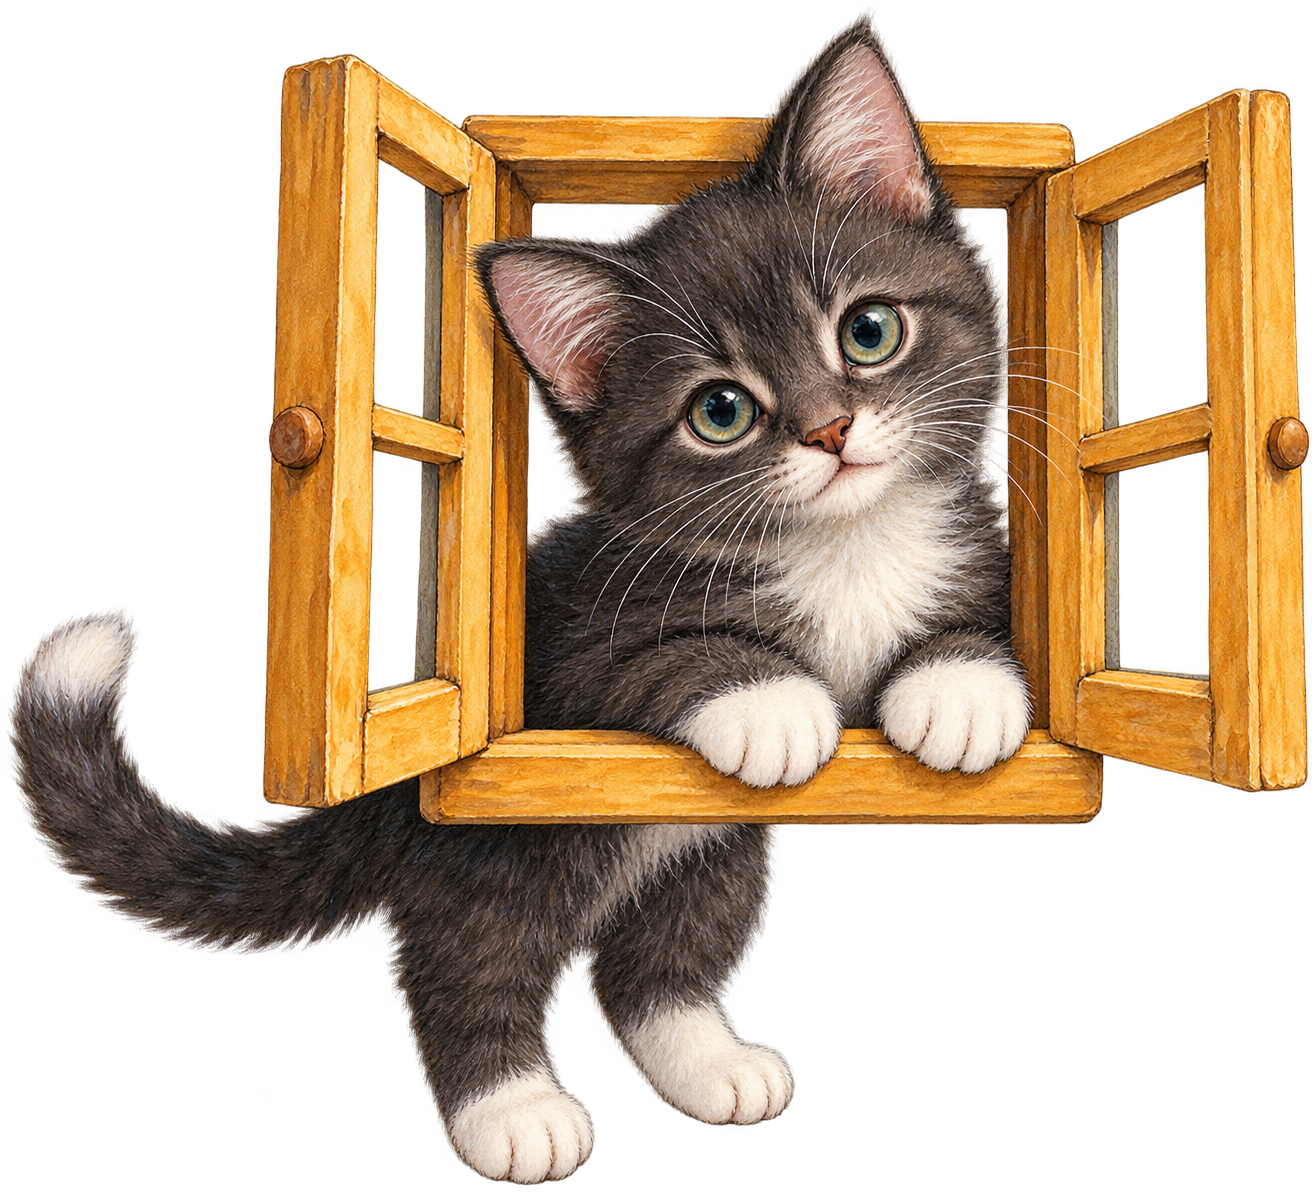
\includegraphics[width=54mm,height=58mm,keepaspectratio]{images/unique/art-245.png}
\end{wrapfigure}
\textit{Доказательство.} Площади \(ABD,ACD\) относятся как \(\frac{BD}{DC}\), поскольку высоты к прямой \(BC\) одинаковы. По формуле площади через две стороны и угол то же отношение равно \(\frac{AB\sin\angle BAD}{AC\sin\angle DAC}=\frac{AB}{AC}\). В \(BIC\) углы при \(B,C\) равны половинам исходных; вычитание их суммы из \(180^\circ\) даёт вторую формулу.\hfill\(\blacksquare\)
\par\WFclear\end{minipage}\end{lrbox}%
\ifdim\dimexpr\ht\CatFlowBox+\dp\CatFlowBox\relax<58mm\dp\CatFlowBox=\dimexpr58mm-\ht\CatFlowBox\relax\fi%
\noindent\usebox{\CatFlowBox}\par\addvspace{2pt}

\begin{example}\textbf{Разбор 3: не смешивать центры.} При \(AB=10,AC=15,BC=20\) биссектриса из \(A\) делит основание как \(2:3\): \(BD=8,DC=12\). Медиана из той же вершины делит основание на \(10,10\). В отдельной задаче при длине медианы \(18\) её отрезки до и после центроида равны \(12,6\). Биссектриса и медиана здесь различны, поскольку стороны \(AB,AC\) не равны. Центроид лежит на медиане, а инцентр — на биссектрисе.\end{example}

\section{Четырёхугольники: свойства и достаточные признаки}
\par\addvspace{2pt}\begin{lrbox}{\CatFlowBox}\begin{minipage}[t]{\linewidth}
\setlength{\parskip}{2pt}\setlength{\columnsep}{4.5mm}\setlength{\intextsep}{0pt}
\begin{wrapfigure}[11]{l}{54mm}

\includegraphics[width=54mm,height=58mm,keepaspectratio]{images/unique/art-243.png}
\end{wrapfigure}
При работе с четырёхугольником полезно отделять название фигуры от признака, по которому это название удалось установить. Если уже известно, что перед нами параллелограмм, можно использовать деление диагоналей пополам. Если же дан только произвольный четырёхугольник, это деление сначала нужно доказать. Похожая осторожность нужна с ромбом: его стороны равны, но диагонали обычно имеют разные длины. У прямоугольника диагонали равны, хотя соседние стороны могут различаться. Когда задача просит доказать, что фигура является квадратом, удобно получить два независимых свойства: прямой угол и равенство соседних сторон. Тогда каждый шаг имеет ясную цель, а случайное внешнее сходство рисунка с квадратом больше не влияет на доказательство.
\par\WFclear\end{minipage}\end{lrbox}%
\ifdim\dimexpr\ht\CatFlowBox+\dp\CatFlowBox\relax<58mm\dp\CatFlowBox=\dimexpr58mm-\ht\CatFlowBox\relax\fi%
\noindent\usebox{\CatFlowBox}\par\addvspace{2pt}
\begin{definition}\term{Параллелограмм} (\emph{parallelogram}) — четырёхугольник с попарно параллельными противоположными сторонами.
\par\term{Прямоугольник} (\emph{rectangle}) — параллелограмм с прямым углом.
\par\term{Ромб} (\emph{rhombus}) — параллелограмм с равными соседними сторонами.
\par\term{Квадрат} (\emph{square}) — одновременно прямоугольник и ромб.
\par\term{Трапеция} (\emph{trapezoid}) здесь имеет ровно одну пару параллельных противоположных сторон, называемых основаниями; остальные стороны — боковые.
\par\term{Равнобедренная трапеция} (\emph{isosceles trapezoid}) имеет равные боковые стороны.\end{definition}
\begin{theorem}[Параллелограмм и его признаки]\label{thm:exam-plane-parallelogram}
У параллелограмма противоположные стороны и углы равны, соседние углы в сумме дают \(180^\circ\), диагонали делятся точкой пересечения пополам. Для признания четырёхугольника параллелограммом достаточно любого условия: обе пары противоположных сторон равны; одна пара противоположных сторон одновременно равна и параллельна; диагонали делятся пополам.
\end{theorem}
\begin{proof}Диагональ параллелограмма разбивает его на равные треугольники по стороне и двум прилежащим углам; отсюда равенство противоположных сторон и углов. У пересечения диагоналей равенство треугольников с вертикальными и накрест лежащими углами даёт половины диагоналей. Сумма соседних углов следует из параллельности.
Обратно, при двух парах равных сторон треугольники по разные стороны диагонали равны по трём сторонам, и равные накрест лежащие углы дают параллельность обеих пар сторон. При одной равной параллельной паре используем равенство треугольников по двум сторонам и углу между ними. При делении диагоналей пополам равны треугольники с вершиной в точке пересечения по двум сторонам и вертикальному углу; снова получаем параллельность.\end{proof}
\begin{theorem}[Прямоугольник, ромб и квадрат]
Параллелограмм является прямоугольником ровно тогда, когда его диагонали равны. Он является ромбом ровно тогда, когда диагонали перпендикулярны; диагонали ромба делят его углы пополам. Если диагональ параллелограмма делит угол пополам, это также признак ромба. Ромб с равными диагоналями является квадратом.
\end{theorem}
\begin{proof}В прямоугольнике Пифагор даёт равные диагонали. Обратно, при \(AC=BD\) треугольники \(DAB,CBA\) равны по трём сторонам; соседние углы \(DAB,ABC\) равны, а их сумма \(180^\circ\), значит, каждый прямой. У ромба треугольники по стороны диагонали равны по трём сторонам, поэтому диагональ делит углы пополам; её половины и половины второй диагонали образуют равные треугольники, смежные углы при пересечении прямые. Обратно, перпендикулярные диагонали параллелограмма дают равные прямоугольные треугольники по катетам, поэтому соседние стороны равны. Если \(AC\) делит угол \(A\), в треугольнике \(DAB\) биссектриса \(AO\) делит \(DB\) пополам; теорема о биссектрисе даёт \(AD=AB\). Последнее утверждение объединяет два уже доказанных признака.\end{proof}
\begin{theorem}[Средняя линия и симметрия трапеции]\label{thm:exam-plane-trapezoid}
Средняя линия трапеции параллельна основаниям и равна их полусумме. Диагональ делит её на отрезки, равные половинам оснований. У равнобедренной трапеции углы при каждом основании равны и диагонали равны; каждое из этих свойств обратно характеризует равнобедренность.
\end{theorem}
\begin{proof}Пусть \(AB\parallel CD\), \(M,N\) — середины боковых сторон \(AD,BC\), а \(K\) — середина \(AC\). Средние линии треугольников \(ADC,ABC\) дают \(MK\parallel CD\), \(KN\parallel AB\), \(MK=\frac{CD}{2}\), \(KN=\frac{AB}{2}\). Значит, \(M,K,N\) лежат на одной прямой.
Для остальных свойств выберем координаты \(A=(0,0),B=(a,0),D=(u,h),C=(u+b,h)\), где \(a,b,h>0\), \(a\ne b\). Равенство боковых сторон означает \(u^2+h^2=(a-b-u)^2+h^2\), откуда \(u=\frac{a-b}{2}\). Тогда фигура симметрична относительно прямой \(x=\frac{a}{2}\); углы и диагонали равны. Равенство углов при основании даёт равенство боковых сторон по общей высоте и синусу равных углов. Равенство диагоналей даёт \((u+b)^2+h^2=(a-u)^2+h^2\), снова \(u=\frac{a-b}{2}\).\end{proof}
\begin{example}\textbf{Разбор 4: диагональ и средняя линия.} Основания трапеции равны \(8,18\). Средняя линия равна \(13\), но диагональ делит её не пополам: части равны \(4,9\). Дополнительное построение — отметить середину самой диагонали. Она связывает две средние линии треугольников; именно поэтому в ответе появляются половины отдельных оснований.\end{example}
\begin{center}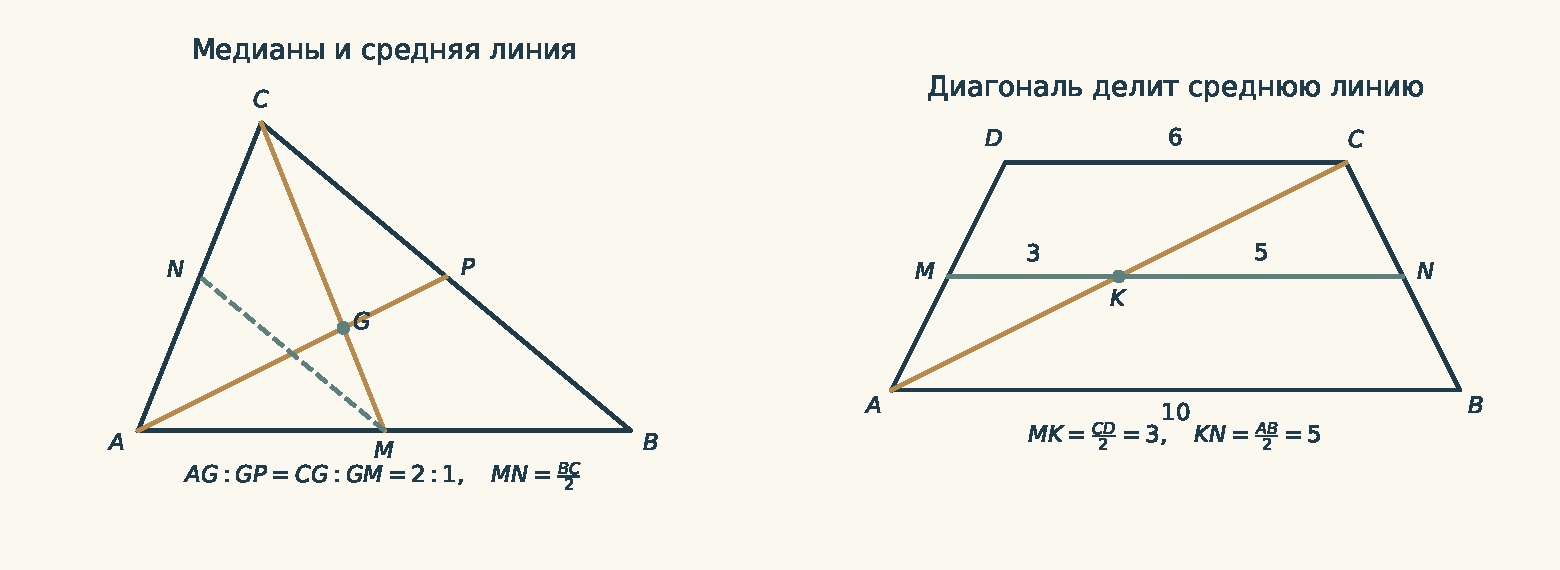
\includegraphics[width=\linewidth]{images/exam-geometry-plane.pdf}\end{center}


\section{Окружности и четырёхугольники}
\begin{definition}\term{Вписанный четырёхугольник} (\emph{cyclic quadrilateral}) имеет все вершины на одной окружности.
\par\term{Описанный четырёхугольник} (\emph{tangential quadrilateral}) имеет окружность внутри, касающуюся всех четырёх сторон, а не только их продолжений.\end{definition}
\begin{theorem}[Признак вписанного четырёхугольника]\label{thm:exam-plane-cyclic}
Четырёхугольник вписан в окружность ровно тогда, когда сумма противоположных углов \(180^\circ\). В частности, трапеция вписана в окружность ровно тогда, когда равнобедренна.
\end{theorem}
\par\addvspace{2pt}\begin{lrbox}{\CatFlowBox}\begin{minipage}[t]{\linewidth}
\setlength{\parskip}{2pt}\setlength{\columnsep}{4.5mm}\setlength{\intextsep}{0pt}
\begin{wrapfigure}[9]{r}{54mm}
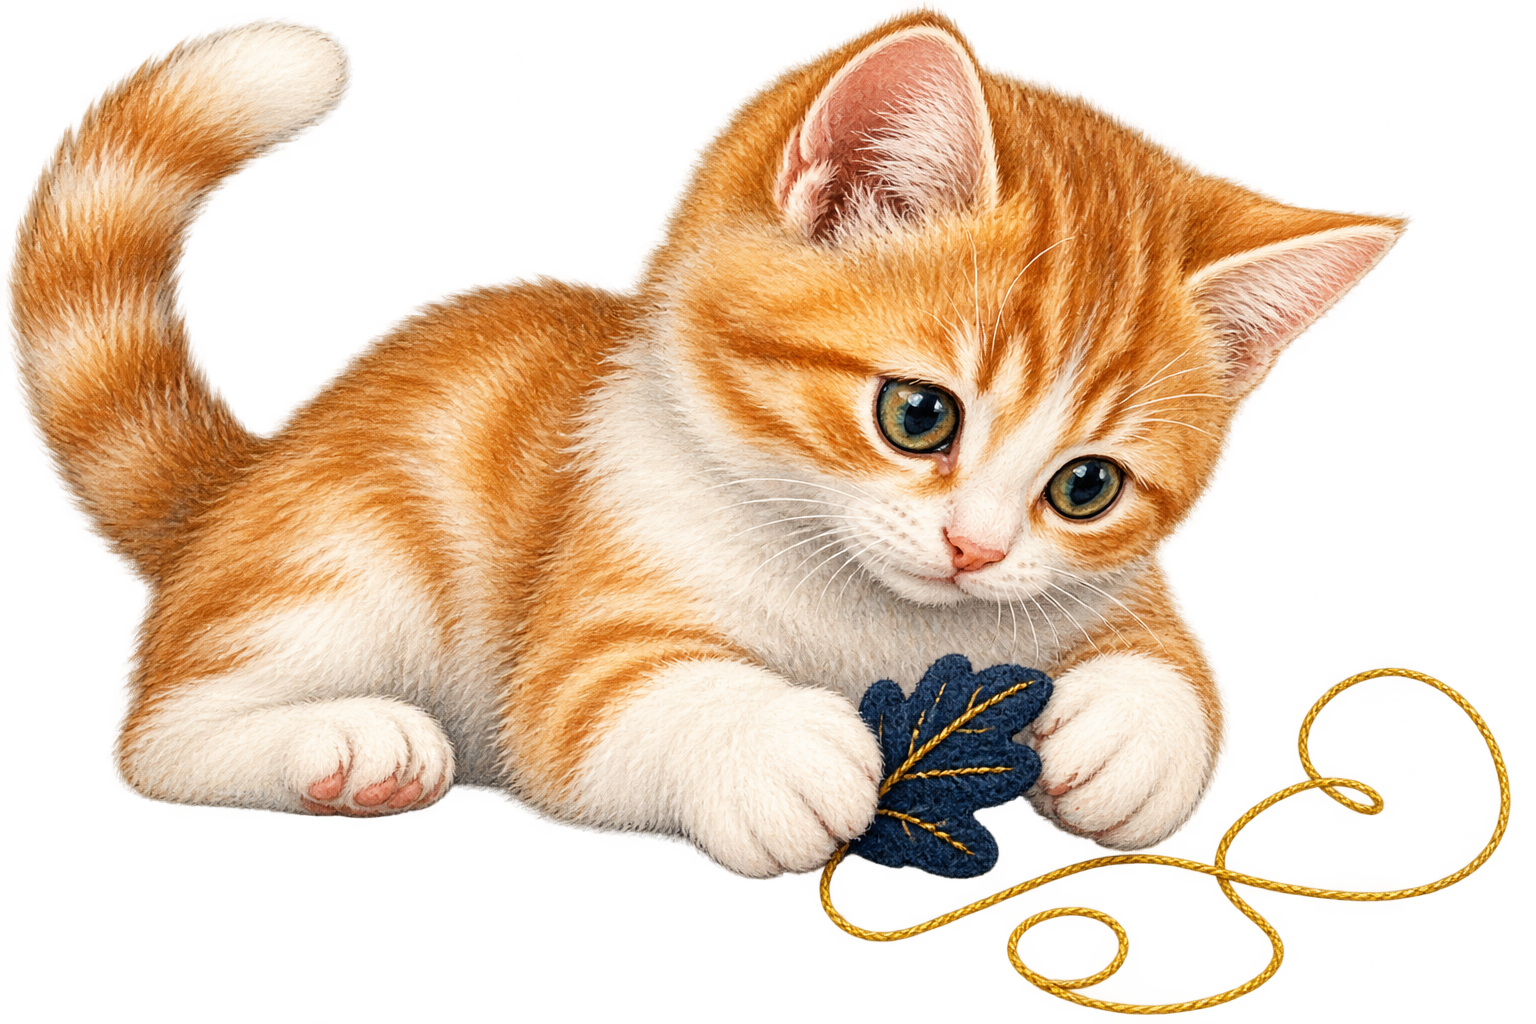
\includegraphics[width=54mm,height=58mm,keepaspectratio]{images/unique/art-258.png}
\end{wrapfigure}
\textit{Доказательство.} Вписанные противоположные углы опираются на две дуги, вместе составляющие \(360^\circ\); сумма половин равна \(180^\circ\). Для обратного утверждения используем следствие теоремы о вписанном угле: по одну сторону данной хорды точки, из которых она видна под заданным углом, образуют дугу одной окружности. Это следствие можно получить построением равнобедренного треугольника из двух радиусов: угол между радиусом и хордой определяет положение центра на её серединном перпендикуляре. Для противоположной стороны хорды дополнительный угол определяет вторую дугу той же окружности. Применим это к диагонали \(AC\) и углам \(ABC,ADC\). В трапеции углы при одной боковой стороне уже дают \(180^\circ\), поэтому условие для противоположных углов равносильно равенству углов при основании, то есть равнобедренности.\hfill\(\blacksquare\)
\par\WFclear\end{minipage}\end{lrbox}%
\ifdim\dimexpr\ht\CatFlowBox+\dp\CatFlowBox\relax<58mm\dp\CatFlowBox=\dimexpr58mm-\ht\CatFlowBox\relax\fi%
\noindent\usebox{\CatFlowBox}\par\addvspace{2pt}

\begin{theorem}[Касательные отрезки и вписанная окружность четырёхугольника]
Если четырёхугольник описан около окружности, то \(AB+CD=BC+DA\). Для окружности достаточно найти внутреннюю точку с одним и тем же положительным расстоянием до четырёх прямых сторон и проверить, что основания перпендикуляров лежат на сторонах. В ромб можно вписать окружность; в прямоугольник это возможно ровно тогда, когда он квадрат.
\end{theorem}
\begin{proof}Из одной внешней точки касательные отрезки к окружности равны по Пифагору, поскольку имеют общую гипотенузу к центру и равные радиусы. Обозначив эти длины у четырёх вершин через \(x,y,z,t\), получим стороны \(x+y,y+z,z+t,t+x\) и нужную сумму. Во втором утверждении круг с указанным центром и радиусом лежит во всех четырёх внутренних полуплоскостях и касается нужных отрезков. В ромбе диагонали делят углы пополам, поэтому их пересечение равноудалено от всех сторон, а основания перпендикуляров принадлежат сторонам; получаем вписанную окружность. В прямоугольнике расстояния от равноудалённой от противоположных сторон точки равны половинам двух соседних сторон. Общий радиус возможен лишь при равных сторонах; для квадрата центр диагоналей подходит.\end{proof}
Не следует объявлять произвольный четырёхугольник описанным только на основании красивой картинки. В задаче с найденным центром нужно проверить все четыре касания, включая принадлежность точек касания отрезкам.
\begin{theorem}[Угол касательной и хорды]
Углы между хордой и двумя противоположными лучами касательной в её конце равны половинам мер соответствующих двух дуг между концами хорды; эти углы дополнительны.
\end{theorem}
\begin{proof}Пусть меньшая центральная дуга \(AB\) имеет меру \(\theta\le180^\circ\). В равнобедренном \(OAB\) угол между радиусом \(OA\) и хордой равен \(\frac{180^\circ-\theta}{2}\). Касательная перпендикулярна \(OA\), поэтому один из двух углов равен \(\frac{\theta}{2}\); второй равен \(180^\circ-\frac{\theta}{2}\), то есть половине большей дуги. Для диаметра обе величины \(90^\circ\).\end{proof}
\begin{example}\textbf{Разбор 5: выбор дуги и луча.} Меньшая дуга \(AB\) равна \(100^\circ\). Между хордой \(AB\) и двумя лучами касательной получаются \(50^\circ\) и \(130^\circ\); без выбора луча единственного угла нет. Если в другом вписанном четырёхугольнике \(A=72^\circ,B=105^\circ\), то \(C=108^\circ,D=75^\circ\). Проверка: все четыре угла дают \(360^\circ\).\end{example}

\section{Преобразования и дополнительные построения}
\par\addvspace{2pt}\begin{lrbox}{\CatFlowBox}\begin{minipage}[t]{\linewidth}
\setlength{\parskip}{2pt}\setlength{\columnsep}{4.5mm}\setlength{\intextsep}{0pt}
\begin{wrapfigure}[13]{r}{54mm}
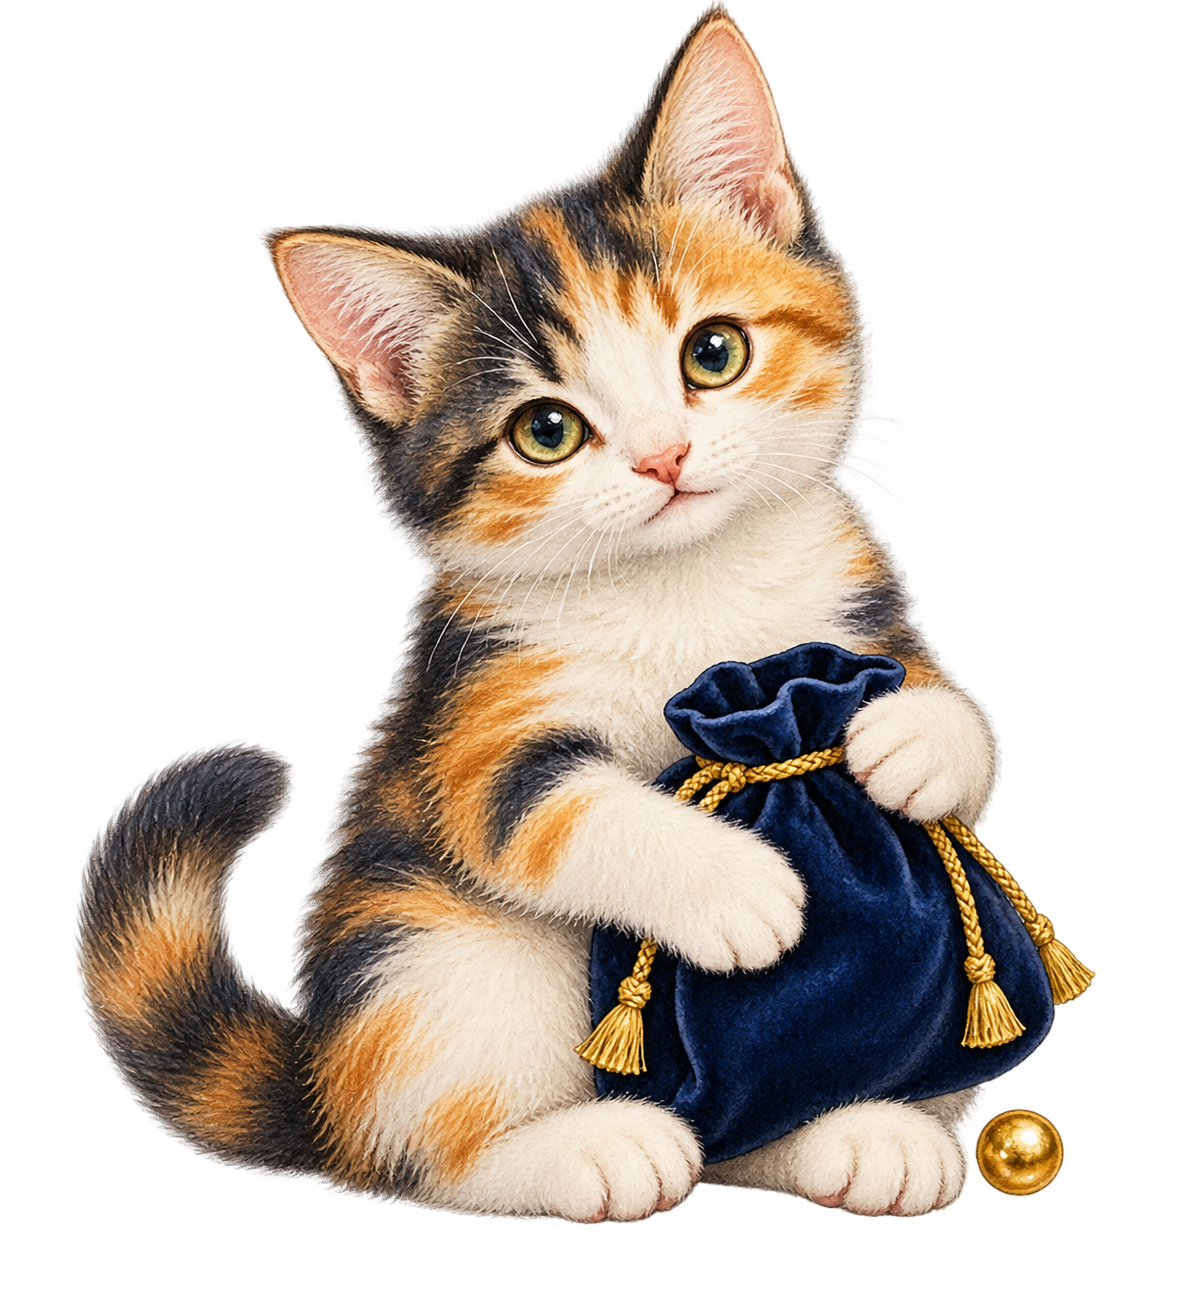
\includegraphics[width=54mm,height=58mm,keepaspectratio]{images/unique/art-244.png}
\end{wrapfigure}
Дополнительная линия особенно полезна, когда она превращает скрытое условие в знакомую фигуру. Через середину стороны можно провести параллель, чтобы получить среднюю линию. Из центра окружности можно опустить радиус в точку касания, чтобы появился прямоугольный треугольник. В задаче с двумя высотами стоит поискать общую окружность по двум прямым углам. При этом построенная точка обязана существовать: две параллельные прямые не пересекутся, а две окружности не всегда имеют общую точку. После построения полезно отдельно проверить, какие равенства следуют из определения новой точки, а какие ещё предстоит доказать. Такой порядок экономит вычисления и делает длинное решение понятным даже без точного масштаба рисунка.
\par\WFclear\end{minipage}\end{lrbox}%
\ifdim\dimexpr\ht\CatFlowBox+\dp\CatFlowBox\relax<61mm\dp\CatFlowBox=\dimexpr61mm-\ht\CatFlowBox\relax\fi%
\noindent\usebox{\CatFlowBox}\par\addvspace{2pt}
\begin{definition}\term{Движение плоскости} (\emph{plane isometry}) сохраняет расстояния.
\par\term{Параллельный перенос} (\emph{translation}) прибавляет к координатам одну фиксированную пару чисел.
\par\term{Осевая симметрия} (\emph{reflection}) относительно прямой оставляет её точки на месте, а остальные меняет с зеркальными так, что прямая — серединный перпендикуляр к соединяющему отрезку.
\par\term{Центральная симметрия} (\emph{point reflection}) с центром \(O\) задаётся условием, что \(O\) — середина \(PP'\).
\par\term{Поворот} (\emph{rotation}) с центром \(O\) сохраняет \(OP\) и увеличивает направленный угол каждого луча \(OP\) на одну величину.
\par\term{Гомотетия} (\emph{homothety}) с центром \(O=(u,v)\) и коэффициентом \(k\ne0\) задаёт \(P'=(u+k(x-u),v+k(y-v))\) для \(P=(x,y)\). При \(k<0\) образ находится на противоположном луче.\end{definition}
\begin{theorem}[Что сохраняет преобразование]
Перенос, симметрии и поворот являются движениями и сохраняют обычные величины углов, параллельность и перпендикулярность. Гомотетия умножает длины на \(|k|\), площади на \(k^2\), сохраняет углы и переводит прямую, не проходящую через центр, в параллельную ей. Прямая через центр переходит в себя.
\end{theorem}
\begin{proof}У переноса разности координат не меняются; у отражения в координатной оси меняется лишь знак одной разности, у центральной симметрии — обеих, поэтому формула расстояния сохраняется. Произвольную ось можно выбрать координатной. Для поворота формула косинусов в \(OPQ\) сохраняет \(PQ\). Углы восстанавливаются по трём длинам, а параллельность — по равным соответствующим углам. При гомотетии обе разности координат умножаются на \(k\); расстояния — на \(|k|\). Подобие треугольников с общей вершиной в центре даёт параллельность образов сторон, а произведение основания и высоты даёт множитель \(k^2\) для площади.\end{proof}
\begin{example}\textbf{Разбор 6: построить и проверить.} Требуется построить треугольник \(ABC\), где \(AB=8,AC=5,BC=7\). Строим \(AB\), окружности с центрами \(A,B\) радиусов \(5,7\), берём одну точку пересечения \(C\). Они пересекаются в двух точках, поскольку \(|7-5|<8<7+5\); выбор полуплоскости делает ответ единственным. Для построения инцентра пересекаем внутренние биссектрисы двух углов и опускаем перпендикуляр к стороне. Равноудалённость доказывает касание также двух остальных сторон. Для серединного перпендикуляра к отрезку используют две окружности одинакового радиуса больше половины его длины: прямая через их пересечения равноудалена от концов.\end{example}
В доказательной задаче достаточно обосновать каждое использованное свойство. Не требуется проводить все возможные линии. Если цель — подобие, выпишем две пары углов; если цель — касание, проверим перпендикулярность радиуса; если цель — вид четырёхугольника, назовём конкретный достаточный признак.

\relax

\par\addvspace{2pt}\begin{lrbox}{\CatFlowBox}\begin{minipage}[t]{\linewidth}
\setlength{\parskip}{2pt}\setlength{\columnsep}{4.5mm}\setlength{\intextsep}{0pt}
\begin{wrapfigure}[13]{r}{54mm}

\includegraphics[width=54mm,height=58mm,keepaspectratio]{images/unique/art-270.png}
\end{wrapfigure}
В задаче с доказательной и вычислительной частями результат первой части обычно создаёт связь, которой не хватало для вычисления. Это может быть параллельность, равенство углов, цикличность четырёхугольника или отношение длин. При выборе дополнительной точки надо указать, почему она существует и лежит на нужном отрезке или продолжении. Координаты дают другой язык того же доказательства: после выбора осей каждое условие должно превратиться в уравнение, а найденная точка обязана удовлетворять геометрическим ограничениям. Симметрия рисунка помогает выбрать обозначения, но сама по себе не доказывает равенство отрезков. Следующие решения связывают несколько фактов в одну проверяемую цепочку.
\par\WFclear\end{minipage}\end{lrbox}%
\ifdim\dimexpr\ht\CatFlowBox+\dp\CatFlowBox\relax<61mm\dp\CatFlowBox=\dimexpr61mm-\ht\CatFlowBox\relax\fi%
\noindent\usebox{\CatFlowBox}\par\addvspace{2pt}
\relax
\section{Дополнительное построение как часть полного решения}
\begin{example}[Диагонали трапеции и её высота]\label{ex:review-ege-exam-plane-1}
У трапеции \(ABCD\), \(AD\parallel BC\), сумма оснований \(10\), диагонали \(AC=6,BD=8\). Докажем их перпендикулярность и найдём высоту. Перенесём отрезок \(BD\) вектором \(\overrightarrow{BC}\): образ точки \(B\) есть \(C\), образ \(D\) — точка \(E\) на прямой \(AD\). Тогда \(CE\parallel BD\), \(CE=8\), а \(AE=AD+BC=10\), причём \(E\) лежит за \(D\). Треугольник \(ACE\) имеет стороны \(6,8,10\), поэтому прямой угол при \(C\). Значит, \(AC\perp BD\). Его площадь \(24\). Высота из \(C\) к \(AE\) одновременно является высотой трапеции: \(h=\frac{2\cdot24}{10}=\frac{24}{5}\). Тот же результат получается из площади трапеции \(\frac{AD+BC}{2}h\). Перенос соединил данные о двух диагоналях в одном треугольнике.
\end{example}

\begin{example}[Касательные, диаметр и ось симметрии]\label{ex:review-ege-exam-plane-2}
Из внешней точки \(N\) к окружности центра \(O\) проведены касательные \(NA,NB\); \(BC\) — диаметр. Пусть \(AB=8,AC=6\). Угол \(BAC\) прямой, поэтому \(BC=10\), радиус \(R=5\). Так как \(NA=NB\), \(OA=OB\), прямая \(NO\) — серединный перпендикуляр к \(AB\). Одновременно \(AC\perp AB\); следовательно, \(AC\parallel NO\).
Пусть \(H\) — середина \(AB\). Из прямоугольного \(OHA\): \(AH=4\), \(OH=3\). Треугольник \(OAN\) прямоугольный при \(A\), поэтому основание его высоты \(H\) лежит внутри гипотенузы \(ON\). Прямоугольные треугольники \(OHA\), \(OAN\) подобны по углу при \(O\), поэтому \(\frac{OH}{OA}=\frac{OA}{ON}\). Отсюда \(ON=\frac{25}{3}\). Направление луча проверено, а не угадано по рисунку.
\end{example}

\begin{example}[Две высоты и расстояние до хорды]\label{ex:review-ege-exam-plane-3}
В остроугольном \(ABC\) основания высот \(BE,CF\) лежат на \(AC,AB\). Пусть \(EF=10\), \(\angle A=60^\circ\). Поскольку \(\angle BEC=\angle BFC=90^\circ\), точки \(B,C,E,F\) лежат на окружности с диаметром \(BC\). Для вычисления стороны удобно другое подобие: \(AE=AB\cos A\), \(AF=AC\cos A\), угол \(EAF=A\), значит, треугольники \(AEF\) и \(ABC\) подобны с соответствием \(E\leftrightarrow B,F\leftrightarrow C\) и коэффициентом \(\cos A\). Поэтому \(EF=BC\cos A\), \(BC=20\). Радиус окружности, описанной около исходного \(ABC\), равен \(R=\frac{20}{2\sin60^\circ}=\frac{20}{\sqrt3}\). Расстояние от её центра до хорды \(BC\):
\[
d=\sqrt{R^2-\frac{BC^2}{4}}=\frac{10}{\sqrt3}.
\]
Окружность через основания высот и окружность исходного треугольника здесь разные: нельзя подставлять радиус одной вместо радиуса другой.
\end{example}
\section{Две внешне касающиеся окружности}
\par\addvspace{2pt}\begin{lrbox}{\CatFlowBox}\begin{minipage}[t]{\linewidth}
\setlength{\parskip}{2pt}\setlength{\columnsep}{4.5mm}\setlength{\intextsep}{0pt}
\begin{wrapfigure}[13]{r}{54mm}
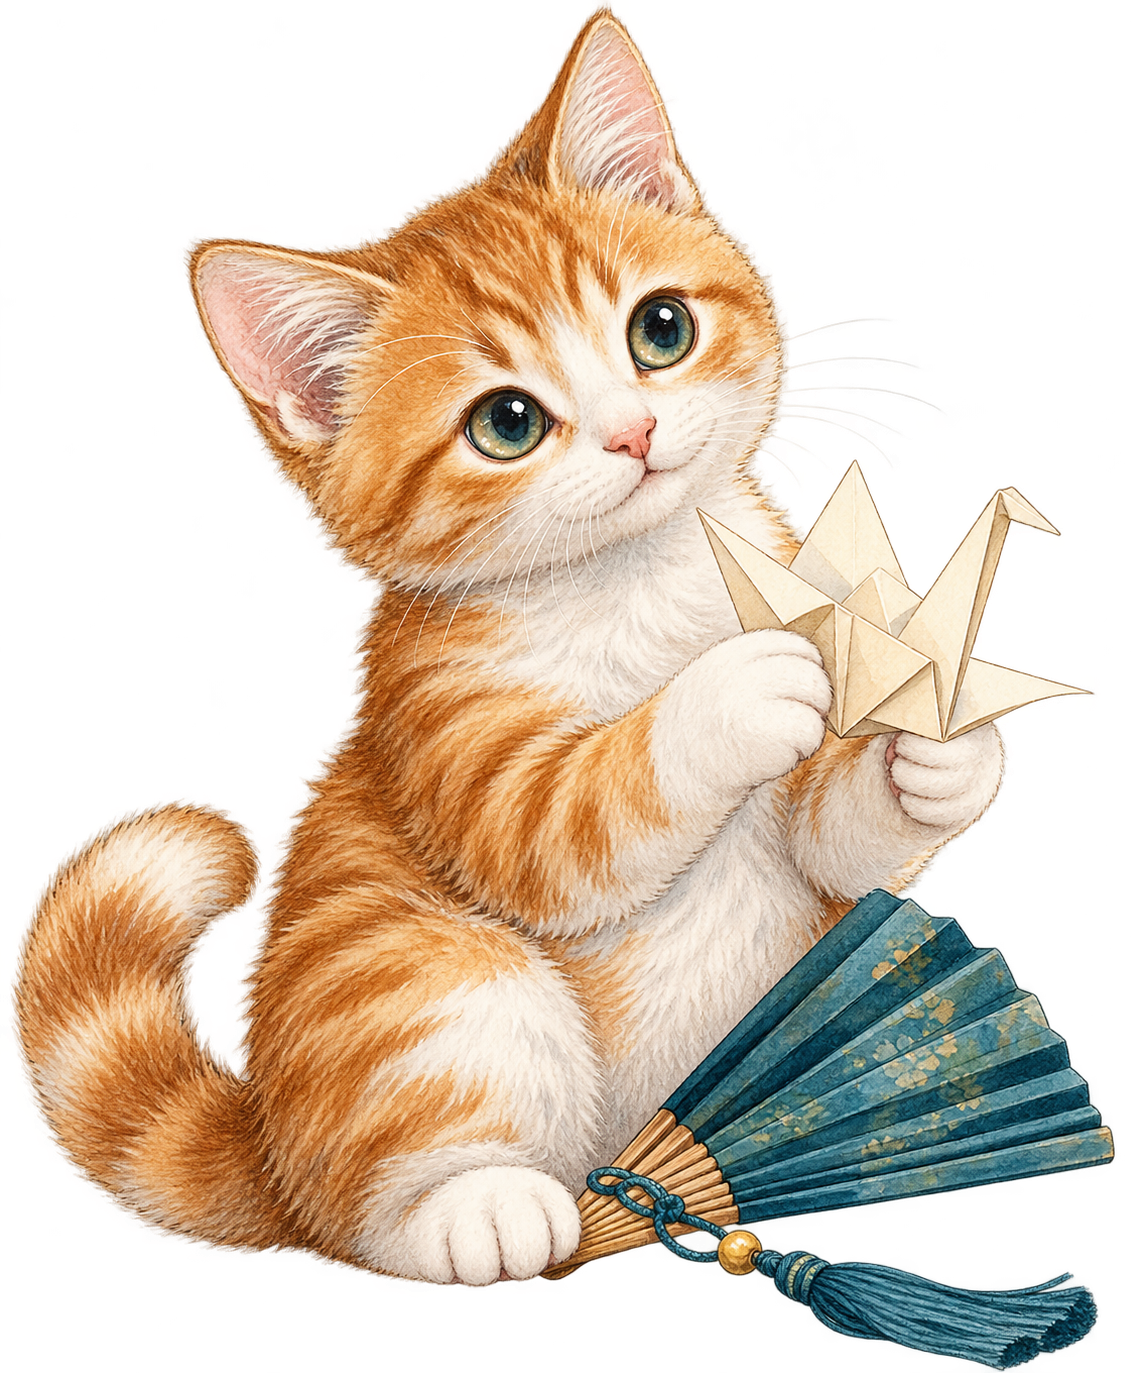
\includegraphics[width=54mm,height=58mm,keepaspectratio]{images/unique/art-284.png}
\end{wrapfigure}
У двух внешне касающихся окружностей есть общая точка, но нет общей внутренней области. Радиусы, проведённые в точку касания, лежат на одной прямой, поэтому касательная в этой точке перпендикулярна линии центров. При различных радиусах выбор общей внешней касательной даёт прямоугольный треугольник, один катет которого равен модулю разности радиусов. Отношения отрезков удобнее находить после этого построения, а не по виду рисунка. Если касательная пересекает линию центров вне окружностей, отдельно проверяют порядок точек. Равенства длин касательных действуют для отрезков из одной внешней точки, а формулы для секущих требуют сохранить длину от внешней точки до дальнего пересечения.
\par\WFclear\end{minipage}\end{lrbox}%
\ifdim\dimexpr\ht\CatFlowBox+\dp\CatFlowBox\relax<61mm\dp\CatFlowBox=\dimexpr61mm-\ht\CatFlowBox\relax\fi%
\noindent\usebox{\CatFlowBox}\par\addvspace{2pt}
\relax

\begin{example}[Общая касательная превращает угол в прямой]\label{ex:review-ege-targeted-tangent-circles}
Окружности радиусов \(R=9\) и \(r=4\) внешним образом касаются в \(K\). Их общая внешняя касательная касается большей окружности в \(A\), меньшей --- в \(B\). Прямая \(BK\) второй раз пересекает большую окружность в \(D\), а прямая \(AK\) второй раз пересекает меньшую в \(C\). Докажем \(\angle AKB=90^\circ\), \(AD\parallel BC\) и найдём площадь \(AKB\).

Проведём общую касательную к окружностям в \(K\); пусть она пересекает \(AB\) в \(M\). Из равенства касательных из одной точки получаем \(MA=MK\) для первой окружности и \(MB=MK\) для второй. Значит, \(MA=MB=MK\), причём на прямой \(AB\) точка \(M\), равноудалённая от \(A,B\), --- середина \(AB\). Таким образом, \(K\) лежит на окружности с диаметром \(AB\); угол \(AKB\) прямой. Поскольку \(B,K,D\) коллинеарны, вписанный угол \(AKD\) также прямой и \(AD\) --- диаметр большей окружности. Аналогично \(BC\) --- диаметр меньшей. Оба диаметра перпендикулярны касательной \(AB\), поэтому параллельны.

Для вычисления выберем \(AB\) осью абсцисс: \(A=(0,0)\), \(B=(L,0)\), центры \(O_1=(0,R)\), \(O_2=(L,r)\) находятся по одну сторону общей внешней касательной. Расстояние центров равно \(R+r\), откуда
\[
L^2+(R-r)^2=(R+r)^2,
\qquad L=2\sqrt{Rr}=12.
\]
Точка внешнего касания лежит на отрезке центров и делит его в отношении \(O_1K:KO_2=R:r\). Значит, её расстояние до \(AB\) равно
\[
h=\frac{rR+Rr}{R+r}=\frac{72}{13}.
\]
Следовательно,
\[
S_{AKB}=\frac12Lh=\frac{432}{13}.
\]
Прямой угол и параллельность получены из касательных и вписанных углов; координаты потребовались лишь для вычисления площади.
\end{example}

\section{Вписанный пятиугольник: две трапеции и подобие}
\begin{example}[Пересечение диагоналей связывает два набора хорд]\label{ex:review-ege-targeted-pentagon}
Точки \(A,B,C,D,E\) в указанном порядке образуют выпуклый вписанный пятиугольник. Пусть \(AB=CD=2\), \(BC=DE=3\), \(AD=4\). Докажем \(AC=BD=CE\) и найдём \(BE\).

Равные хорды \(AB,CD\) стягивают равные вписанные углы: \(\angle BCA=\angle CAD\). Следовательно, \(BC\parallel AD\). Из \(BC=DE\) аналогично \(\angle CDB=\angle DBE\), значит, \(CD\parallel BE\). Четырёхугольник \(ABCD\) --- равнобедренная трапеция с основаниями \(AD,BC\), поэтому \(AC=BD\). Четырёхугольник \(BCDE\) --- равнобедренная трапеция с основаниями \(BE,CD\), поэтому \(BD=CE\).

Пусть \(M=AD\cap BE\). Диагонали выпуклого четырёхугольника \(ABDE\) пересекаются внутри обоих отрезков. Из найденных параллельностей \(BCDM\) --- параллелограмм, откуда
\[
BM=CD=2,\qquad MD=BC=3,\qquad AM=AD-MD=1.
\]
Углы \(BAM=BAD\) и \(MED=BED\) опираются на одну хорду \(BD\), а \(\angle BMA=\angle DME\) вертикальны. Поэтому \(\triangle ABM\sim\triangle EDM\), с соответствием \(A\leftrightarrow E\), \(B\leftrightarrow D\). Тогда
\[
\frac{AM}{ME}=\frac{BM}{MD}=\frac23,
\qquad ME=\frac32,
\qquad BE=BM+ME=\frac72.
\]
Положение \(M\) внутри отрезков определило, где нужны сумма, а где разность длин.
\end{example}

\section{Две высоты параллелограмма: координаты после площади}
\begin{example}[Условия на высоты определяют вторую сторону]\label{ex:review-ege-targeted-parallelogram}
В параллелограмме \(ABCD\) основания перпендикуляров \(BP\perp AD\), \(BQ\perp CD\) лежат на отрезках \(AD,CD\). На \(AD\) взята точка \(M\), причём \(AM=BP=4\), \(AB=BQ=5\). Докажем \(BM=PQ\) и найдём площадь \(APQ\).

Положим \(A=(0,0)\), направим ось абсцисс вдоль \(AD\), а \(B\) расположим над ней. Из прямоугольного \(ABP\) имеем \(AP=\sqrt{25-16}=3\), поэтому \(B=(3,4)\), \(P=(3,0)\), \(M=(4,0)\). Площадь параллелограмма можно выразить через любую сторону и соответствующую высоту:
\[
AD\cdot BP=CD\cdot BQ=AB\cdot BQ=25,
\qquad AD=\frac{25}{4}.
\]
Значит, \(D=(\frac{25}{4},0)\), \(C=(\frac{37}{4},4)\). Прямая \(CD\) параллельна \(AB\), её уравнение \(4x-3y=25\). Перпендикуляр к ней через \(B\) имеет уравнение \(3x+4y=25\). Их пересечение \(Q=(7,1)\). Эта точка действительно лежит на \(CD\): \(Q=D+\frac14(C-D)\).

Теперь
\[
BM=\sqrt{(4-3)^2+(0-4)^2}=\sqrt{17},
\qquad PQ=\sqrt{(7-3)^2+(1-0)^2}=\sqrt{17},
\]
а основание \(AP=3\) лежит на оси абсцисс, высота из \(Q\) равна \(1\). Поэтому \(S_{APQ}=\frac32\). Использованы и метрическое условие о высотах, и проверка положения основания \(Q\).
\end{example}

\section{Медианы и весь след прямой в треугольнике}
\par\addvspace{2pt}\begin{lrbox}{\CatFlowBox}\begin{minipage}[t]{\linewidth}
\setlength{\parskip}{2pt}\setlength{\columnsep}{4.5mm}\setlength{\intextsep}{0pt}
\begin{wrapfigure}[13]{l}{54mm}

\includegraphics[width=54mm,height=58mm,keepaspectratio]{images/unique/art-285.png}
\end{wrapfigure}
Медианная конструкция переводится в координаты без вычисления всех длин треугольника. Середина стороны задаётся полусуммой координат её концов, а любая точка прямой через две известные точки выражается через один параметр. После нахождения пересечения надо проверить, где лежит параметр: принадлежность прямой не означает принадлежности отрезку. Условие о середине или отношении частей часто сокращает уравнения раньше вычислений. Поэтому сначала записывают именно отношения, которые даёт конструкция, и только затем ищут координаты неизвестной точки. Полученная алгебраическая запись должна сохранить названия вершин и направление выбранной параметризации; иначе верное отношение можно ошибочно отнести к другой стороне.
\par\WFclear\end{minipage}\end{lrbox}%
\ifdim\dimexpr\ht\CatFlowBox+\dp\CatFlowBox\relax<61mm\dp\CatFlowBox=\dimexpr61mm-\ht\CatFlowBox\relax\fi%
\noindent\usebox{\CatFlowBox}\par\addvspace{2pt}
\relax

\begin{example}[Точка пересечения не является концом искомого отрезка]\label{ex:review-ege-targeted-medians}
В прямоугольном \(ABC\), \(\angle C=90^\circ\), \(AC=3\), \(BC=4\), точки \(M,N\) --- середины \(AB,BC\). На \(BC\) выбрана \(K\) с \(CK:KB=1:3\), \(P=AN\cap KM\). Докажем \(AN=2KM\) и найдём длину отрезка, который прямая \(BP\) высекает внутри треугольника.

Возьмём \(C=(0,0)\), \(B=(4,0)\), \(A=(0,3)\). Тогда \(M=(2,\frac32)\), \(N=(2,0)\), \(K=(1,0)\). По формуле расстояния
\[
AN=\sqrt{13},\qquad KM=\frac{\sqrt{13}}2,
\]
что доказывает требуемое отношение. Для нахождения \(P\) запишем точки отрезков:
\[
AN:\ (x,y)=(2t,3-3t),\qquad
KM:\ (x,y)=(1+s,\frac32s),\quad0\le t,s\le1.
\]
Из \(2t=1+s\), \(3-3t=\frac32s\) получаем \(t=\frac34\), \(s=\frac12\), то есть \(P=(\frac32,\frac34)\). Точка \(P\) лежит внутри треугольника, поэтому искомый след не равен \(BP\): прямая продолжается до второй стороны. Её точки имеют вид
\[
(x,y)=(4,0)+\lambda(-\frac52,\frac34).
\]
На стороне \(AC\) абсцисса нулевая, поэтому \(\lambda=\frac85\), \(T=(0,\frac65)\). Так как \(0<\frac65<3\), точка \(T\) принадлежит стороне \(AC\). Выпуклость треугольника означает, что весь след прямой --- отрезок \(BT\), длина которого
\[
BT=\sqrt{4^2+(\frac65)^2}=\frac{2\sqrt{109}}5.
\]
Восстановление обоих концов следа обязательно: вычисление одного \(BP\) решило бы другую задачу.
\end{example}

\section{Окружность у боковых сторон и высоты}
\par\addvspace{2pt}\begin{lrbox}{\CatFlowBox}\begin{minipage}[t]{\linewidth}
\setlength{\parskip}{2pt}\setlength{\columnsep}{4.5mm}\setlength{\intextsep}{0pt}
\begin{wrapfigure}[12]{r}{54mm}

\includegraphics[width=54mm,height=58mm,keepaspectratio]{images/unique/art-286.png}
\end{wrapfigure}
Окружность, касающаяся двух пересекающихся прямых, имеет центр на одной из биссектрис образованных углов. Выбор нужной биссектрисы определяется положением окружности в задаче. Касание третьей прямой выражается равенством расстояния от центра до неё и радиуса. Эти условия дают алгебраические кандидаты, но не всегда завершают построение: радиус должен быть положительным, центр должен лежать в требуемой области, а точки касания с прямыми могут оказаться на продолжениях сторон. Условие касания стороны как отрезка проверяют отдельно. Симметрия равнобедренного треугольника сокращает число неизвестных, однако не отменяет проверки положения окружности относительно высоты и основания.
\par\WFclear\end{minipage}\end{lrbox}%
\ifdim\dimexpr\ht\CatFlowBox+\dp\CatFlowBox\relax<61mm\dp\CatFlowBox=\dimexpr61mm-\ht\CatFlowBox\relax\fi%
\noindent\usebox{\CatFlowBox}\par\addvspace{2pt}
\relax

\begin{example}[Биссектрисы дают вписанный четырёхугольник]\label{ex:review-ege-targeted-altitude-circle}
В равнобедренном остроугольном \(ABC\), \(AB=BC\), проведена высота \(CH\) к \(AB\). Окружность с центром \(O\) вписана в прямоугольный треугольник \(BHC\); таким образом, она касается боковых сторон \(AB,BC\) и отрезка высоты \(CH\). Пусть \(AC=8\), \(BO=3\). Докажем \(\angle OAC=45^\circ\) и найдём \(BC\).

Обозначим равные углы при основании через \(\alpha\). Так как исходный треугольник остроугольный, \(45^\circ<\alpha<90^\circ\). В прямоугольном \(BHC\)
\[
\angle BCH=90^\circ-\angle CBH
=90^\circ-(180^\circ-2\alpha)=2\alpha-90^\circ.
\]
Центр вписанной окружности лежит на биссектрисах: \(CO\) делит этот угол пополам, поэтому \(\angle BCO=\alpha-45^\circ\), а \(\angle ACO=45^\circ\). Биссектриса прямого угла при \(H\) даёт \(\angle OHC=45^\circ\), \(\angle AHO=135^\circ\). Сумма противоположных углов \(AHO\), \(ACO\) равна \(180^\circ\), следовательно, \(A,H,O,C\) лежат на одной окружности. Теперь углы, опирающиеся на хорду \(OC\), равны:
\[
\angle OAC=\angle OHC=45^\circ.
\]

Из \(\angle OAC=\angle ACO=45^\circ\) также \(\angle AOC=90^\circ\). Пусть \(M\) --- середина \(AC\). Медиана прямоугольного \(AOC\), проведённая к гипотенузе, даёт \(OM=\frac{AC}{2}=4\). Центр \(O\) лежит на биссектрисе угла \(B\), то есть на высоте \(BM\) исходного равнобедренного треугольника. Он расположен внутри \(BHC\), поэтому между \(B\) и \(M\). Следовательно,
\[
BM=BO+OM=7,\qquad
BC=\sqrt{BM^2+MC^2}=\sqrt{65}.
\]
Касание именно отрезков трёх сторон прямоугольного треугольника выбрало вписанную окружность и исключило окружности, касающиеся продолжений.
\end{example}
\Needspace{7\baselineskip}\section*{Задачи}
\begingroup\setlength{\parskip}{0pt}
\noindent\begin{minipage}[t]{\linewidth}\textbf{29.1.} При пересечении прямых один угол равен \(37^\circ\). Найди остальные три.\par\end{minipage}\par
\noindent\begin{minipage}[t]{\linewidth}\textbf{29.2.} Односторонние внутренние углы при двух параллельных прямых равны \(3x+10^\circ\) и \(5x+10^\circ\). Найди \(x\) и углы.\par\end{minipage}\par
\noindent\begin{minipage}[t]{\linewidth}\textbf{29.3.} В равнобедренном треугольнике угол между равными сторонами равен \(40^\circ\). Найди углы при основании и обоснуй равенство этих углов.\par\end{minipage}\par
\noindent\begin{minipage}[t]{\linewidth}\textbf{29.4.}\starmark{} Медиана \(AM\) треугольника \(ABC\) перпендикулярна \(BC\). Докажи \(AB=AC\).\par\end{minipage}\par
\noindent\begin{minipage}[t]{\linewidth}\textbf{29.5.}\starmark{} Два прямоугольных треугольника имеют равные гипотенузы и один соответствующий катет. Докажи равенство треугольников без дополнительного чертежа.\par\end{minipage}\par
\par\addvspace{2pt}\begin{lrbox}{\CatFlowBox}\begin{minipage}[t]{\linewidth}
\setlength{\parskip}{2pt}\setlength{\columnsep}{4.5mm}\setlength{\intextsep}{0pt}
\begin{wrapfigure}[12]{r}{54mm}
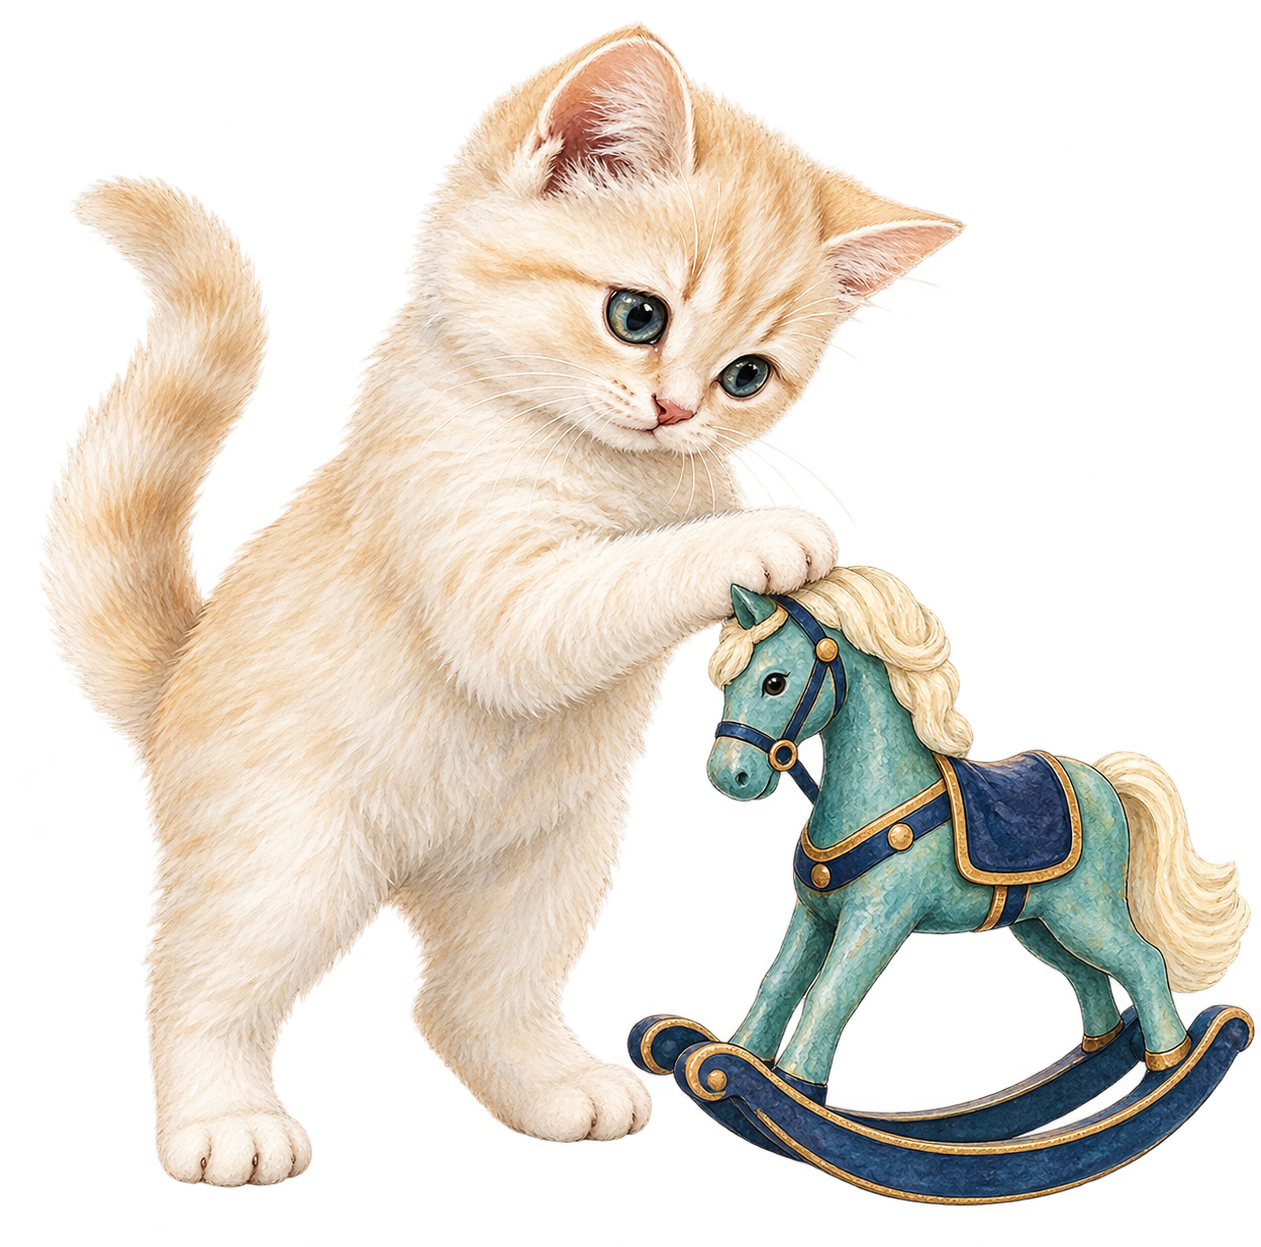
\includegraphics[width=54mm,height=58mm,keepaspectratio]{images/unique/art-246.png}
\end{wrapfigure}
\textbf{29.6.} Две стороны треугольника равны \(5,8\). Какие целые значения может иметь третья сторона?\par

\textbf{29.7.} В прямоугольном \(ABC\) катеты \(AC=6,BC=8\), \(CH\) — высота к гипотенузе. Найди \(AB,AH,BH,CH\).\par

\textbf{29.8.} В \(ABC\) даны \(AB=6,AC=9,BC=10\); \(AD\) — внутренняя биссектриса. Найди \(BD,DC\).\par

\textbf{29.9.} Медиана \(AM\) равна \(12\), \(G\) — центроид. Найди \(AG,GM\).\par
\par\WFclear\end{minipage}\end{lrbox}%
\ifdim\dimexpr\ht\CatFlowBox+\dp\CatFlowBox\relax<58mm\dp\CatFlowBox=\dimexpr58mm-\ht\CatFlowBox\relax\fi%
\noindent\usebox{\CatFlowBox}\par\addvspace{2pt}

\noindent\begin{minipage}[t]{\linewidth}\textbf{29.10.} Угол \(A\) равен \(70^\circ\), \(I\) — инцентр. Найди \(\angle BIC\).\par\end{minipage}\par
\noindent\begin{minipage}[t]{\linewidth}\textbf{29.11.}\starmark{} Через вершины треугольника проведены прямые, параллельные противоположным сторонам. Объясни, почему центр описанной окружности полученного внешнего треугольника — ортоцентр исходного.\par\end{minipage}\par
\noindent\begin{minipage}[t]{\linewidth}\textbf{29.12.} Найди центр и радиус окружности через \(A=(0,0),B=(4,0),C=(1,1)\). Лежит ли центр внутри треугольника?\par\end{minipage}\par
\noindent\begin{minipage}[t]{\linewidth}\textbf{29.13.}\starmark{} У двух треугольников равны углы между сторонами \(4,6\) и \(6,9\). Докажи подобие и найди коэффициент от первого ко второму.\par\end{minipage}\par
\noindent\begin{minipage}[t]{\linewidth}\textbf{29.14.} Стороны двух треугольников равны \(3,4,5\) и \(6,8,10\). Найди отношение их площадей и назови достаточный признак подобия.\par\end{minipage}\par
\noindent\begin{minipage}[t]{\linewidth}\textbf{29.15.}\starmark{} Середины сторон \(AB,AC\) треугольника соединены отрезком \(MN\), \(BC=14\). Докажи \(MN\parallel BC\) и найди \(MN\).\par\end{minipage}\par
\noindent\begin{minipage}[t]{\linewidth}\textbf{29.16.} Основания трапеции равны \(6,14\). Найди среднюю линию и части, на которые её делит диагональ.\par\end{minipage}\par
\noindent\begin{minipage}[t]{\linewidth}\textbf{29.17.}\starmark{} Диагонали выпуклого \(ABCD\) пересекаются в \(O\), причём \(AO=OC,BO=OD\). Докажи, что \(ABCD\) — параллелограмм.\par\end{minipage}\par
\noindent\begin{minipage}[t]{\linewidth}\textbf{29.18.}\starmark{} В выпуклом \(ABCD\) стороны \(AB,CD\) равны и параллельны. Докажи параллельность \(AD,BC\).\par\end{minipage}\par
\noindent\begin{minipage}[t]{\linewidth}\textbf{29.19.} У параллелограмма обе диагонали равны \(10\), сторона равна \(3\). Докажи, что он прямоугольник, и найди другую сторону.\par\end{minipage}\par
\noindent\begin{minipage}[t]{\linewidth}\textbf{29.20.} У ромба диагонали равны \(10,24\). Найди сторону, площадь и радиус вписанной окружности.\par\end{minipage}\par
\noindent\begin{minipage}[t]{\linewidth}\textbf{29.21.}\starmark{} Докажи: ромб с равными диагоналями является квадратом. Достаточно ли равенства диагоналей для произвольного четырёхугольника?\par\end{minipage}\par
\noindent\begin{minipage}[t]{\linewidth}\textbf{29.22.} В равнобедренной трапеции основания равны \(4,14\), боковая сторона \(13\). Найди высоту и площадь.\par\end{minipage}\par
\noindent\begin{minipage}[t]{\linewidth}\textbf{29.23.}\starmark{} Докажи, что трапеция с равными углами при одном основании равнобедренна.\par\end{minipage}\par
\noindent\begin{minipage}[t]{\linewidth}\textbf{29.24.} Вписанный четырёхугольник имеет углы \(A=75^\circ,B=110^\circ\). Найди \(C,D\).\par\end{minipage}\par
\noindent\begin{minipage}[t]{\linewidth}\textbf{29.25.}\starmark{} Докажи, что трапеция, вписанная в окружность, равнобедренна.\par\end{minipage}\par
\noindent\begin{minipage}[t]{\linewidth}\textbf{29.26.} Четырёхугольник \(ABCD\) описан около окружности. Даны \(AB=3,BC=4,CD=7\). Найди \(DA\).\par\end{minipage}\par
\noindent\begin{minipage}[t]{\linewidth}\textbf{29.27.} Можно ли вписать окружность в прямоугольник со сторонами \(8,12\)? Обоснуй.\par\end{minipage}\par
\noindent\begin{minipage}[t]{\linewidth}\textbf{29.28.} Меньшая дуга \(AB\) имеет меру \(130^\circ\). Найди оба угла между хордой \(AB\) и лучами касательной в \(A\).\par\end{minipage}\par
\noindent\begin{minipage}[t]{\linewidth}\textbf{29.29.} Найди образы \(P=(3,-2)\) при отражении относительно оси \(x\) и при центральной симметрии относительно \(O=(1,1)\).\par\end{minipage}\par
\noindent\begin{minipage}[t]{\linewidth}\textbf{29.30.} Точку \(P=(2,-3)\) повернули на \(90^\circ\) против часовой стрелки около начала координат, затем перенесли на \((-1,4)\). Найди итоговую точку.\par\end{minipage}\par
\noindent\begin{minipage}[t]{\linewidth}\textbf{29.31.} Гомотетия имеет центр \((1,-1)\) и коэффициент \(-2\). Найди образ \((4,2)\), длину образа отрезка длины \(5\) и площадь образа фигуры площади \(7\).\par\end{minipage}\par
\noindent\begin{minipage}[t]{\linewidth}\textbf{29.32.}\starmark{} Опиши построение треугольника \(ABC\) с \(AB=5\), \(AC=6\), \(BC=7\) циркулем и линейкой и докажи существование. Сколько возможных положений вершины \(C\), если отрезок \(AB\) фиксирован?\par\end{minipage}\par
\noindent\begin{minipage}[t]{\linewidth}\textbf{29.33.}\starmark{} Опиши построение вписанной окружности произвольного треугольника. Почему достаточно двух биссектрис?\par\end{minipage}\par
\noindent\begin{minipage}[t]{\linewidth}\textbf{29.34.}\starmark{} В остроугольном \(ABC\) высоты \(BE,CF\) имеют основания \(E\in AC,F\in AB\). Докажи, что \(B,C,E,F\) лежат на одной окружности; укажи полезный диаметр.\par\end{minipage}\par
\noindent\begin{minipage}[t]{\linewidth}\textbf{29.35.} В трапеции \(ABCD\) основания \(AD\parallel BC\). Внутренние биссектрисы углов \(A,B\) пересекаются в \(F\), \(AF=8,BF=6\). Найди \(AB\), обосновав прямой угол.\par\end{minipage}\par
\noindent\begin{minipage}[t]{\linewidth}\textbf{29.36.}\starmark{} Вписанный выпуклый \(ABCD\) имеет пересекающиеся продолжения \(AB,CD\) в \(M\), причём точки расположены в порядке \(M,A,B\) и \(M,D,C\). Докажи подобие \(MBC,MDA\).\par\end{minipage}\par
\noindent\begin{minipage}[t]{\linewidth}\textbf{29.37.}\starmark{} Из внешней точки \(N\) проведены касательные \(NA,NB\) к окружности центра \(O\). Отрезок \(BC\) — диаметр; \(AB=12,AC=5\). Докажи \(AC\parallel NO\) и найди \(NO\).\par\end{minipage}\par
\noindent\begin{minipage}[t]{\linewidth}\textbf{29.38.}\starmark{} В трапеции \(ABCD\), \(AD\parallel BC\), даны \(AB=12,CD=15,BC=3\). Внутренняя биссектриса угла \(D\) проходит через середину \(M\) стороны \(AB\). Найди площадь.\par\end{minipage}\par
\noindent\begin{minipage}[t]{\linewidth}\textbf{29.39.}\starmark{} Сумма оснований трапеции равна \(17\), диагонали равны \(8\) и \(15\). Докажи перпендикулярность диагоналей и найди высоту.\par\end{minipage}\par
\noindent\begin{minipage}[t]{\linewidth}\textbf{29.40.}\starmark{} Из \(N\) проведены касательные \(NA,NB\) к окружности с центром \(O\) и радиусом \(13\); \(BC\) — её диаметр, \(AB=10\). Докажи \(AC\parallel NO\) и найди \(NO\).\par\end{minipage}\par
\noindent\begin{minipage}[t]{\linewidth}\textbf{29.41.}\starmark{} В остроугольном треугольнике \(ABC\) основания высот из \(B,C\) обозначены \(E,F\). Даны \(EF=9\), \(\angle A=45^\circ\). Докажи цикличность \(B,C,E,F\) и найди расстояние от центра описанной около \(ABC\) окружности до стороны \(BC\).\par\end{minipage}\par
\noindent\begin{minipage}[t]{\linewidth}\textbf{29.42.}\starmark{} Две окружности радиусов \(16\) и \(9\) внешним образом касаются в \(K\). Их общая внешняя касательная имеет точки касания \(A,B\). Докажи, что \(\angle AKB=90^\circ\), и найди площадь \(AKB\).\par\end{minipage}\par
\noindent\begin{minipage}[t]{\linewidth}\textbf{29.43.}\starmark{} Выпуклый пятиугольник \(ABCDE\) вписан в окружность; вершины идут по ней в указанном порядке. Известно \(AB=CD=3\), \(BC=DE=4\), \(AD=5\). Докажи \(AC=BD=CE\) и найди \(BE\), указав положение \(M=AD\cap BE\).\par\end{minipage}\par
\noindent\begin{minipage}[t]{\linewidth}\textbf{29.44.}\starmark{} В параллелограмме \(ABCD\) основания высот \(BP\perp AD\), \(BQ\perp CD\) лежат на соответствующих отрезках. Точка \(M\in AD\), \(BP=AM=12\), \(AB=BQ=13\). Докажи \(BM=PQ\), найди эту общую длину и площадь \(APQ\).\par\end{minipage}\par
\noindent\begin{minipage}[t]{\linewidth}\textbf{29.45.}\starmark{} В прямоугольном \(ABC\), \(\angle C=90^\circ\), \(AC=5\), \(BC=12\), точки \(M,N\) --- середины \(AB,BC\). Точка \(K\in BC\) удовлетворяет \(CK:KB=1:3\), \(P=AN\cap KM\). Докажи \(AN=2KM\) и найди длину всего отрезка прямой \(BP\), лежащего в треугольнике.\par\end{minipage}\par
\noindent\begin{minipage}[t]{\linewidth}\textbf{29.46.}\starmark{} В равнобедренном остроугольном \(ABC\), \(AB=BC\), высота \(CH\) опущена на \(AB\). Окружность с центром \(O\) вписана в прямоугольный \(BHC\). Известно \(AC=10\), \(BO=7\). Докажи \(\angle OAC=45^\circ\) и найди \(BC\).\par\end{minipage}\par
\endgroup
